\documentclass[10pt,letterpaper]{article}
\usepackage[letterpaper,margin=0.5cm]{geometry}
\usepackage[utf8]{inputenc}
\usepackage{amsmath}
\usepackage{amsfonts}
\usepackage{pdfpages}
\usepackage{amssymb}
\usepackage{siunitx}
\author{Jeffrey Wubbenhorst}
\title{Math 216 Midterm 2 Study Guide }

\begin{document}
\maketitle

\section*{Dimension, Linear Indepence} 
\subsection*{Subspaces and Spanning Sets }% chap 2.2
\begin{itemize}

\item A subset $W$ of a vector space $BV$ is a subspace of $V$ if $W$ is a subspace under addition, scalar multiplication of $V$ restricted to  $W$. (That is, if $W$ is closed under the same rules of scalar mulitplication and addition as $V$)

\item Let $W$ be a nonempty subset of a vector space $V$. $W$ is a subspace of $V$ iff, $\forall u, v \in W$ and $\forall c \in \mathbb{R}, u + w \in W, cu \in W$
% do I need to translate this into English tho 

\item If $A$ is $m\times n$, solutions to system of homogenous linear equations $AX=0$ is a subspace of $\mathbb{R}^n$

\item A set of vectors $\{v_1, v_2, ..., v_n$ is \textbf{linearly independent }iff, for a system $c_1v_1+c_2v_2+...+c_nv_n=0$ all constants $c$ are zero. As a random note, no set containing hte zero vector is independent. 

\end{itemize}

\subsection*{Dimension, Nullspace, Row Space, Column Space }
% chapt 2.4 
\begin{itemize}

\item If a vector space $V$ has a basis of $n$ vectors, the \textbf{dimension of $V$ is $n$}. This is denoted as $\mbox{dim}(V)$. 

\item $\mbox{dim}(\mathbb{R}^n)=n, \mbox{dim}M_m\times n(\mathbb{R})=mn, \mbox{dim}(P_n)=n+1$


\item Suppose some $v_1, v_2,...v_n$ in a vector space $V$. The vectors are \textbf{linearly dependent} iff \textit{only one} if $v_1,v_2,...,v_n$ is a linear combination of the others. To see if a set of vectors is linearly independent, solve for the constants for the homogenous equation; if a non-trivial solution exists, then the vectors are linearly dependent. 

\item Vectors $v_1,v_2,...,v_n $ of a vector space $V$ are a basis for $V$ if both of the following conditions are satisfied: 
\begin{enumerate}
\item $v_1,v_2,...,v_n$ are \textbf{linearly independent}
\item $v_1, v_2,...,v_n$ \textbf{span} $V$
\end{enumerate}

\item Suppose some $v_1, v_2,...v_n$ in a vector space $V$. Then $v_1, v_2,...,v_n$ form a basis for $V$ iff each vector in $V$ is uniquely expressible as a linear combonation of $v_1,v_2,...,v_n$

\item If $V$ is a bvector space adn $v_1, v_2, ...,v_n$ are vectors in $V$, then the set of all linear combinationfs of $v_1, v_2,...,v_n$ is a subspace of $V$ 

\item The subspace of some $V$ consisting of all linear combinations of vectors $v_1, v_2,...,v_n$ is referred to as the \textbf{subspace} of $V$ spanned by $v_1, v_2,...,v_n$ \\
...in English, the span is the set of all the different places you could ``go" if you combined the given vectors in every possible way. To see if something spans something else, solve for constants $c$; if there's no solution, then the set does not span. 

\item Suppose that $V$ is a vector space of dimension $n$. 
\begin{enumerate}
\item If the vecrtors $v_1,v_2,...,v_n$ are linearly independet, then $v_1,v_2, ...,v_n$ are linearly independent, then $v_1,v_2, ...,v_n$  form a basis for $V$

\item If $v_1,v_2, ...,v_n$ span $V$, then $v_1,v_2, ...,v_n$ form a \textbf{basis}
\end{enumerate}

\item The solutions to the homogenous system $AX=0$, where $A$ is an $m\times n$ matrix form a subspace of $\mathbb{R}^n$. This vector space of solutions is the \textbf{nullspace} or \textbf{kernel}$\mbox{ of } A, \mbox{ denoted by } NS(A)$

\item The \textbf{row space} of some matrix $A$ is the span of the rows of $A$. If $A, B$ are row-equivalent matrices, $RS(A)=RS(B)$

\item Weirdly enough, for an $m\times n \mbox{ matrix },\mbox{dim}(RS(A))+\mbox{dim}(NSA(A))=n$

\item The \textbf{column space} of a matrix $A$ is the subspace of $\mathbb{R}^m$ spanned by the columns of $A$ and is denoted by $CS(A)$. To find the column space of a matrix, you: 
\begin{enumerate}
\item \textbf{T}ranspose 
\item \textbf{R}ow-reduce
\item transpose back 
\item take \textbf{B}asis vectors 
\end{enumerate}
...dumb mnemonic is \textbf{TR}i\textbf{B}e. (Or `tribble' if you're into Star Trek.) 

\item [more weird stuff] For a given matrix $A, \mbox{dim}(RS(A)) = \mbox{dim}(CS(A))$; this common dimension is called the \textbf{rank} of $A$. 

\end{itemize}

\subsection*{Wronskians} % chapter 2.5 

\begin{itemize}
% * internally debates whether or not to actually bother representing what a wronskian is in LaTeX * 
\item Suppose some $f_1, f_2,...,f_n$ are functions in $D^{n-1}(a,b).\mbox{ If the \textbf{Wronskian} }w(f_1(x),f_2(x),...,f_n(x)) \mbox{ of } f_1,f_2,...,f_n$
is nonzero for some $x$ in $(a,b)$, then $f_1, f_2, ...,f_n \mbox{ are linearly independent elements of }D^{n-1}(a,b)$
% add in Bray's thing !!! 

\end{itemize}


% 4.3 
\section*{Differential Equations}

\subsection*{Complex Solutions}
\begin{itemize}

\item if $L(y)=0$ is a CCLDE w/ real coefficientsr and if $y(x) = \mu(x) + iv(x)$ is a complex-valued solution, $\mu(x), v(x)$ are also solutions. 

\item If $L(y)=0$ is a real CCLDE and $r, \bar{r}$ are a pair of roots of characteristic polynomial, then 
$e^{ax}\cos bx, e^{ax}s\sin bx$ are real, independent solutions, with same span as $e^{rx}, e^{\bar{r}x}$

\item If $L(Y)=0$ has a characteristic polynomial with roots $r_1, ...,r_n$, and sets of solutions formed by: 
\begin{enumerate}
\item For real roots $r$ of multiplicity $m$, we include 
$$e^{rx}, xe^{rx}, ..., x^{m-1}e^{rx}$$
\item For complex roots $r$ of multiplicity $m$, we include
 $$e^{rx}\cos bx, e^{rx}\sin bx, xe^{rx}\cos bx, xe^{rx}\sin bx , ..., x^{m-1}e^{rx}\cos bx, x^{m-1}e^{rx}\sin bx$$
\end{enumerate}
...then this set of functions is independent, and is a fundamental set of solutions. 


\end{itemize}



\subsection*{Method of Undetermined Coefficients}
\begin{itemize}
\item The solution to a differential equation is the sum of the particular solution and the homogenous solution: 
$$ y= y_h+y_p$$
\item The goal is to find some $y_p$ that works with some given differential equation, with $\lambda = r$ is a root of multiplicity $m$, $k$ is highest power of $x$ on the right side of the equation. 
\item If the root to an LDE of the form $a_ny^{(n)}+...+a_1y'+a_0y=Ax^ke^{rx}$ is real, the particular solution will be $y_p=x^m(A_kx^k+...+A_1x+A_0)e^{rx}$
\item If root to equation of form 
$$ a_ny^{(n)}+...+a_1y'+a_0y=Ax^ke^{ax}\cos bx+Bx^ke^{ax}\sin bx $$
is imaginary, particular solution is given as: 
$$ y_p = x^m(A_kx^k+...+A_1x+A_0)e^{ax}\cos bx + x^m(B_kx^k+...+B_1x+B_0)e^{ax}\sin bx $$
\item \textit{Note: the method of undetermined coefficients is \underline{not} an exact science!} There can be trial and error involved; a table of decent guesses is embedded at the end of this document. 
\end{itemize}

\subsection*{Applications} % chap 4.5 + errata 
\begin{itemize}
\item Sitautions with no external forces are usually given in the form 
$$F = mu'' + fu' + ku = 0$$
where (in spring problems at least) $k$ is the spring constant, $f$ is the friction coefficient, and mass $m$. (Don't forget that pounds are a unit of force, \textit{not} of mass!)

\item In \textbf{unforced cases} (no external input to system), the quadratic equation can give us roots; the issue of imaginary roots arises (that is, $f^2-4km<0$): 
\begin{enumerate}
\item If no friction ($f=0$), roots are imaginary. These cases are kind of rare. 
\item If $f-4km<0$, $\lambda= -a\pm bi$; in this case, the oscillating thing in question takes a bit to stop moving. This system is \textbf{underdamped}.  
\item If $f-4km>0$, there will be two roots $r_1, r_2 < 0$, solutions will have the form $u=c_1e^{r_1t}+c_2e^{r_2t}$
this system is \textbf{overdamped}. 
\item If $f^2-4km=0$, we have one root $r=\frac{-f}{2m}$ and solutions $u=c_1e^{rt}+c_2te^{rt}$. This system is \textbf{critically damped}, and is the case where the oscillating thing returns to rest within the shortest amount of time. 
\end{enumerate}

\item In \textbf{forced cases}, there are a few possible situations: 
\begin{enumerate}
\item For instances of no friction (system is \textbf{undamped}), the equation will have the form: 
$$\mu'' + ku = h(t)$$
We'll consider a case where $\omega_0\neq \omega$, wher $\omega = \sqrt{k/m}$; complete set of solutions can be obtained by: 
$$\mu_H = c_1\cos\omega_0 t + c_2\sin \omega_0 t$$
$$\mu_P = \frac{a}{\omega_0^2-\omega^2}\cos\omega t$$
...and $\mu = \mu_H+\mu_P$. 
\item \textbf{Resonance} occurs when $\omega = \omega_0$; in these situations, the amplitude increases as time increases. This has been known to cause some kinds of problems. 
% add gain and phase shift stuff in?? 
% add in some photos of what these different scenarios look like 

\end{enumerate}


\end{itemize}


% chapt 5.1 
\section*{Linear Transformations}
\begin{itemize}
\item A function $f$ from a set $X$ to a set $Y$ is denoted as $f : X \to Y$; $X$ is the domain of $f$, $Y$ is called the \textbf{image set }or \textbf{codomain}. The subset ${f(x)| x \in X}$ of Y is called the \textbf{range}, which, in English, means ``all the $f(x)$ that `hit' something in $Y$."

\item If $V$, 	$W$ are vector spaces, a function $T : V \to W$ is called a \textbf{linear transformation} if, for all vectors $u, v \in V$ and all scalars $c$, the following two properties hold: 
\begin{enumerate}
\item $T(u+ v) = T(u) +  T(v)$ 
\item $T(cv) = cT(v)$ 
\end{enumerate}

\item If $T : V \to V$, $T$ is sometimes called a \textbf{linear operator }

% theorem 5.1
\item If $A$ is an $m\times n$ matrix, $T : \mathbb{R}^n \to \mathbb{R}^m $ defined by 
$$T(X) = AX$$ is a linear transformation, but is more commonly called a \textbf{matrix transformation}

\item The differential operator takes derivatives, and is a linear transformation denoted by 
$$ D : D(a, b) \to F(a, b)$$

\item  $\mbox{Int}(f)$ denotes definite integral of a function $f$ over a closed interval $[a,b]$

% theorem 5.2
\item For some \textbf{linear transformation}$T : V \to W$ the following properties hold: 
\begin{enumerate}
\item $T(0)=0$
\item $T(-v)=0T(v) $ for any $v\in V$
\item $T(u-v)=T(u)-T(v)$ for any $u, v \in V$ 
\item $T(c_1v_1+c_2v_2+...+c_kv_k)=c_1T(v_1)+c_2T(v_2)+...+c_kT(v_k)$ for any scalars 
$c_1, c_2,...,c_k$ and any vectors $v_1, v_2,...v_k\in V$
\end{enumerate}

\item To determine what exactly a linear transformation does (assuming you have a set of input vectors by which the behavior of $T$ may be observed): 
\begin{enumerate} 
\item Assume, find, or steal some basis for the domain; this will determine all values of an LT. 
\item Determine the coefficients $c_1, ...,c_n$ for the basis vectors that yield a given output 
\item Determine how $T$ combines the given input vectors to an output vector of form  $[x_0,x_1,...,x_n]$, solving again for coefficients
\end{enumerate}

\item The \textbf{kernel} of $T$, denoted $\mbox{ker}(T)$, is defined as 
$$\mbox{ker}(T)=\{ v\in V | T(v)=0\}$$ 
...in English, the kernel is the set of all vectors that give an output of the zero vector. For matrix transformations, the kernel of the matrix transformation $T(X)=AX$ is the same as the nullspace of $A$: 
$$\mbox{ker}(T)=NS(A)$$ % huhuhuhu 

\item To find a basis for the column space of a matrix, take the transpose (\textbf{T}), reduce (\textbf{R}), transpose (\textbf{T}), split into columns (\textbf{S}), which approximately spells \textbf{ToRToiSe}.

\item Weirdly enough, if $T : V \to W$ is an LT where $V$ is a finite-dimensional vector space, we have that 
$$\mbox{dim(ker}(T)+\mbox{dim(range}(T)) = \mbox{dim}(V)$$

\end{itemize}

% this is pretty cool 
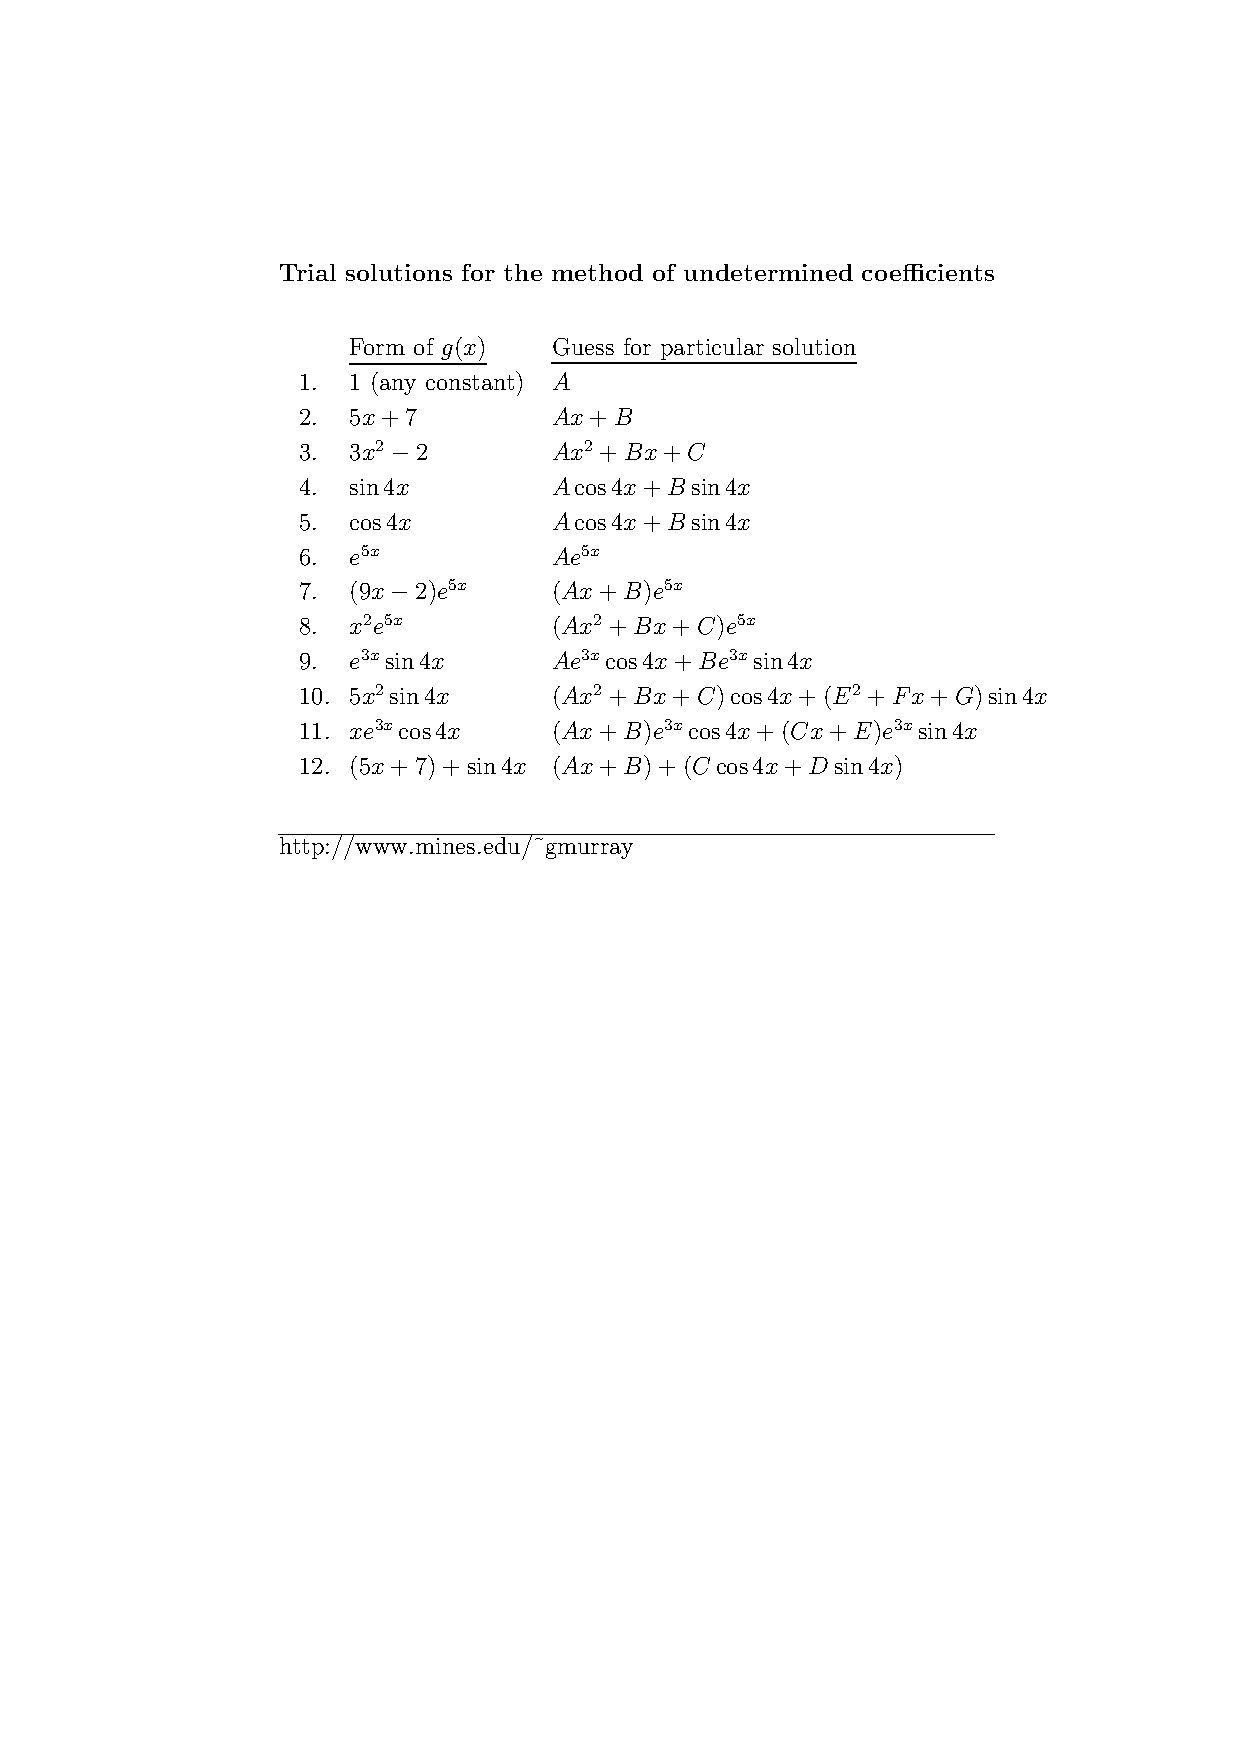
\includepdf[pages={1}]{trialSoln.pdf}


\section*{Errata} 

\begin{itemize}
\item The \textbf{contrapositive }of a statement is the reverse of the premise and conclusion, and the negation of both. Original statement: ``Duke won, and I'm happy." Contrapositive: ``If I'm not happy, then Duke didn't win."
\end{itemize}

\subsection*{Trig Identities}
\begin{itemize}
\item STUFF HERE 
\end{itemize}

\subsection*{Complex stuff!! }
add it yo 


\iffalse 
#### sources 
* http://inside.mines.edu/fs_home/gmurray/teach/s02/trialSoln.pdf

\fi 

\end{document}

